% Lecture file created by newnote
% Class: Models of Theoretical Physics
% Professor: Azaele Sandro
% Date: 2025-10-17
\lecture{4}{Turing Pattern Formation}{2025-10-17}
\pagelayout{margin}
% --- Start writing here ---

\section{Turing Pattern Formation}
Nature offers a wide range of examples of biological patterns, from animal pigmentation to shells, skin, wings and skeletal structures. Patterns are composed of spatially heterogeneous structures which may emerge owing to several (biological) reasons. These could arise in systems in which chemicals react with each other and also underwent diffusion - a mechanism which is termed diffusion-driven instability. This is the basis of the so called Turing patterns.
\begin{figure}[H]
    \centering
    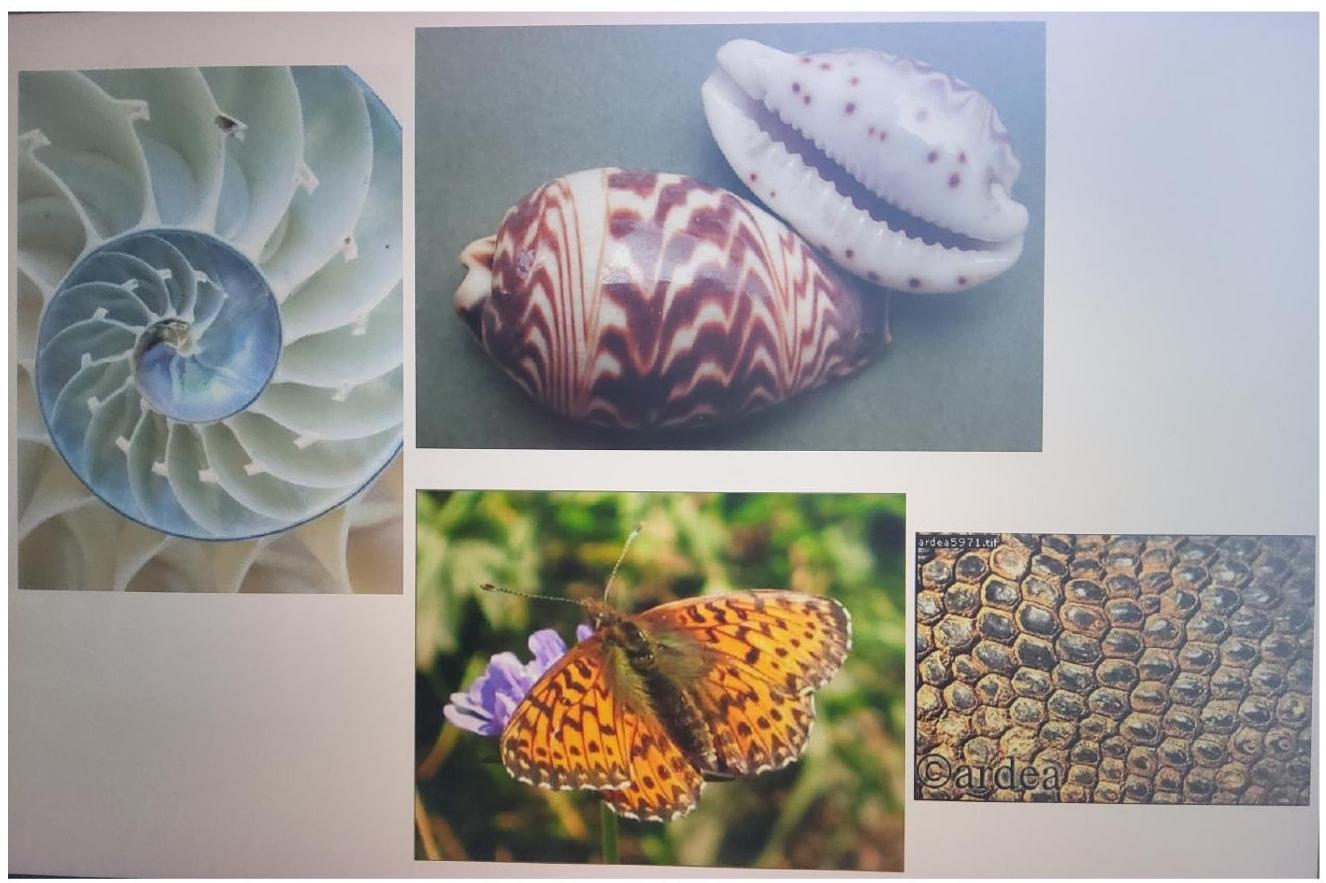
\includegraphics[width=\textwidth]{2025_10_17_3cf351a4349ae3691080g-01}
\end{figure}

Turing patterns and instability are related to symmetry breaking in non-equilibrium systems and represent an example of emergent pattern, namely, a structure that emerges from the combination of processes, which per se do not possess any property related to the pattern itself.

In 1952 Alan Turing (logician, computer scientist, code breaker and mathematician) proposed a mathematical model which was able to show emergent patterns (A.M. Turing, the chemical basis of morphogenesis, Philos. Trans. R. Soc. London B 237, 37-72, (1952)).

Turing showed that when some chemicals react with each other and diffuse appropriately, then spatially heterogeneous patterns can emerge (diffusion-driven instability), if some conditions are met.

\subsection*{One chemical species}
Let us consider the case with one chemical species, diffusing in a one-dimensional space. We could consider the reactions
\begin{DispWithArrows}
    \left.\begin{array}{l}
    3 U \underset{k_{-}}{\stackrel{k_{+}}{\rightleftarrows}} 2 U \\
    \phi \underset{\mu_{-}}{\stackrel{\mu_{+}}{\rightleftarrows}} U
    \end{array}\right\} \rightarrow \dot{u}=-k_{+} u^{3}+k_{-} u^{2}-\mu_{-} u+\mu_{+}

\end{DispWithArrows}
which involve only the species $U$ ($u$ is its concentration).
For the sake of generality, let's assume that the chemical $U$ is being produced at rate $f(u)$ (typically a polynomial or a rational function of $u$). If we include diffusion
\begin{DispWithArrows}[tag=1]
    \frac{\partial u}{\partial t}=D \frac{\partial^{2} u}{\partial x^{2}}+f(u)
\end{DispWithArrows}
Where $D>0$ is the diffusion coefficient. Eq. (1) is a reaction-diffusion equation.
We also assume that $U$ diffuses in a domain $(0,L)$ and that
\begin{DispWithArrows}[tag=2]
    u(0, t)=u_{0}=u(L, t) \quad \forall t
\end{DispWithArrows}
These are called Dirichlet boundary conditions. If there is a spatially uniform stationary state $u_0$ for $u$, then we also have $\lim_{t \to \infty} u(x, t)=u_{0}$ and $f\left(u_{0}
ight)=0$.
Is this state stable? In general this is a hard question, but we can check whether $u_{0}$ is linearly stable. To check this we have to determine the effect of a small perturbation.
$\hat{u}(x, t)=u(x, t)-u_{0} \quad\left(|\hat{u}| \ll u_{0}\right)$. Expanding $f$ in a Taylor series we get (only linear terms) from eq. (1)
\begin{DispWithArrows}[tag=3]
    \frac{\partial \hat{u}}{\partial t}=D \frac{\partial^{2} \hat{u}}{\partial x^{2}}+f^{\prime}\left(u_{0}
ight) \hat{u} \quad \hat{u}(0, t)=0=\hat{u}(L, t)
\end{DispWithArrows}
where we assumed $f\left(u_{0}
ight)=0$ and $f^{\prime}\left(u_{0}
ight) \neq 0$. Without space ($D=0$) we get
\begin{DispWithArrows}[tag=4]
    \hat{u}(x, t)=\hat{u}_{0} e^{f^{\prime}\left(u_{0}
ight) t}
\end{DispWithArrows}
$\hat{u}_{0}$ is the initial perturbation. Of course, the steady state is stable if $f^{\prime}\left(u_{0}
ight)<0$. If $D>0$, then eq. (3) can be solved via separation of variables: $\hat{u}(x, t)=h(x) k(t)$. Thus we get from eq. (3)
\begin{DispWithArrows}
    \begin{aligned}
    \left(\partial_{t} k\right) h & =D k\left(\partial_{x}^{2} h\right)+f^{\prime}\left(u_{0}
ight) k h \\ 
    \frac{\partial_{t} k}{k} & =D \frac{\partial_{x}^{2} h}{h}+f^{\prime}\left(u_{0}
ight)
    \end{aligned}
\end{DispWithArrows}
because the l.h.s. depends on $t$ only and the r.h.s. on $x$ only, it must be
\begin{DispWithArrows}
    \underbrace{\frac{\partial_{t} k}{k}}_{a}=\lambda=\overbrace{D \frac{\partial_{x}^{2} h}{h}+f^{\prime}\left(u_{0}
ight)}^{b}
\end{DispWithArrows}
Where $\lambda$ is constant independent of time and space
a) $\partial_{t} k=\lambda k \Rightarrow k(t)=k_{0} e^{\lambda t}$
b) $\partial_{x x}^{2} h=\underbrace{\frac{\lambda-f^{\prime}\left(u_{0}
ight)}{D}}_{-\rho^{2}} h \Rightarrow h(x)=A \sin (\rho x)+B \cos (\rho x)$

From the B.C. in eq. (2) we obtain $h(0)=0 \Rightarrow B=0$ and also $h(L)=0 \Rightarrow \rho=\frac{n \pi}{L}$ for any $n=1,2 \ldots$
Hence the modes
\begin{DispWithArrows}[tag=5]
    \lambda_{n}=f^{\prime}\left(u_{0}
ight)-D\left(\frac{n \pi}{L}\right)^{2} \quad n=1,2, \cdots
\end{DispWithArrows}
Because the eq. is linear, we can sum all the modes and get the final solution as a Fourier series:
\begin{DispWithArrows}[tag=6]
    \hat{u}(x, t)=\sum_{n=1}^{\infty} a_{n} \sin \left(\frac{n \pi x}{L}\right) e^{\lambda_{n} t} \quad \hat{u}(0, t)=0=\hat{u}(L, t)
\end{DispWithArrows}
where $a_{n}$ are determined to satisfy the initial condition for the pert. Note from (5) that, even if $f^{\prime}\left(u_{0}
ight)>0$ ($u_{0}$ is unstable), then $D>f^{\prime}\left(u_{0}
ight)\left(\frac{L}{\pi}\right)^{2}$ (for fixed domain size L) implies $\lambda_{n}<0$. Therefore, all terms in eq. (6) with $a_{n} \neq 0$ have an expon. decay, hence $\hat{u} \rightarrow 0$ as $t \rightarrow \infty$.
In this case the state $u_{0}$ is stabilized by diffusion, even when it is unstable, if $D$ is sufficiently large. D cannot destabilize the solution.

\subsection*{Exercise:}
If B.C. are zero-flux at the boundaries $\left(\frac{\partial u}{\partial x}(0)=0=\frac{\partial u}{\partial x}(L)\right.$, Neumann B.C.) the zeroth mode could still grow, but all the others decay exponentially so there cannot be any spatial heterogeneity for large $D$. Same arguments still hold for periodic B.C.

Obs: Notice that diffusivity is not always able to stabilize.
If we fix $D$ and increase $L$ when $f^{\prime}\left(u_{0}
ight)>0$, then for sufficiently large domain sizes $\left(L>\sqrt{\frac{D \pi^{2}}{f^{\prime}\left(u_{0}
ight)}}\right)$ we still get $\lambda_{n}>0$. The effect of diffusion depends on the domain.

\subsection*{Two or more chemical species}
From the previous section we have learnt that diffusion is able to smooth out inhomogeneities, thus stabilizing processes. This agrees with other phenomena, e.g., diffusion of heat within a finite domain.
Turing understood that if there are more than one interacting species, this is not necessarily the case and diffusion may destabilize homogeneous solutions.
Let $u(x, t)$ and $v(x, t)$ be the concentrations of two chemical species which satisfy the following reaction-diffusion equations in 1-d space:
\begin{DispWithArrows}[tag=7]
    \left.\begin{array}{l}\dot{u}=f(u, v)+D_{1} \frac{\partial^{2} u}{\partial x^{2}} \\ 
    \dot{v}=g(u, v)+D_{2} \frac{\partial^{2} v}{\partial x^{2}}
    \end{array}\right. \quad \text { with I.C. and B.C.}
\end{DispWithArrows}
where $f$ and $g$ are smooth functions which describe the reactions between the two chemicals whose concentrations are given by $u$ and $v . D_{1}$ and $D_{2}$ are two diffusion constants. We assume that $x \in(0,L)$ (finite domain) and at the boundaries we impose zero-flux conditions (Neumann b.c.).

Let us assume that eq. (7) admits a spatially uniform steady state, hence there exist $u_{0}$ and $v_{0}$ such that $f\left(u_{0}, v_{0}
ight)=0=g\left(u_{0}, v_{0}
ight)$. We now wish to derive conditions of linear stability for the state $\left(u_{0}, v_{0}\right)$. For this we introduce small (spatially-dependent) perturbations $\hat{u}(x, t)=u(x, t)-u_{0}$ and $\hat{v}(x, t)=v(x, t)-v_{0}$ into eq. (7) and expand $f$ and $g$ in Taylor series. We arrive at (recall that $f\left(u_{0}, v_{0}\right)=0, g\left(u_{0}, v_{0}\right)=0$)
\begin{DispWithArrows}[tag=8]
    \left.\begin{array}{l}\dot{\hat{u}}=\left.\frac{\partial f}{\partial u}\right|_{0} \hat{u}+\left.\frac{\partial f}{\partial v}\right|_{0} \hat{v}+D_{1} \frac{\partial^{2} \hat{u}}{\partial x^{2}} \\ 
    \dot{\hat{v}}=\left.\frac{\partial g}{\partial u}\right|_{0} \hat{u}+\left.\frac{\partial g}{\partial v}\right|_{0} \hat{v}+D_{2} \frac{\partial^{2} \hat{v}}{\partial x^{2}}
    \end{array}\right.
\end{DispWithArrows}
where $\left.\left.\frac{\partial f}{\partial u}\right|_{0} \equiv \frac{\partial f(u, v)}{\partial u}\right|_{\substack{u=u_{0} \ v=v_{0}}}$ and the same for the rest. We can recast eq. (8) in the matrix form
\begin{DispWithArrows}
    \binom{\partial_{t} \hat{u}}{\partial_{t} \hat{v}}=\underbrace{\left(\begin{array}{cc}
    \left.\frac{\partial f}{\partial u}\right|_{0} & \left.\frac{\partial f}{\partial v}\right|_{0} \\ 
    \left.\frac{\partial g}{\partial u}\right|_{0} & \frac{\partial g}{\left.\partial v\right|_{0}}
    \end{array}\right)}_{\equiv J_{0}}\binom{\hat{u}}{\hat{v}}+\underbrace{\left(\begin{array}{cc}
    D_{1} & 0 \\ 
    0 & D_{2}
    \end{array}\right)}_{\equiv D}\binom{\partial_{x}^{2} \hat{u}}{\partial_{x}^{2} \hat{v}}
\end{DispWithArrows}
or
\begin{DispWithArrows}[tag=9]
    \frac{\partial}{\partial t} \overrightarrow{\hat{u}}=J_{0} \overrightarrow{\hat{u}}+D \partial_{x}^{2} \overrightarrow{\hat{u}}
\end{DispWithArrows}
We carry out the analysis of the previous section and look for a solution of the form
\begin{DispWithArrows}[tag=10]
    \vec{u}(x, t)=\vec{a} e^{\left(i k x+\lambda\left(k^{2}
ight) t\right)}
\end{DispWithArrows}
where $\vec{a}$ is a constant vector. Subbing (10) into (9) we get
\begin{DispWithArrows}
    \lambda \vec{a} e^{i k x+\lambda t}=J_{0} \vec{a} e^{i k x+\lambda t}-k^{2} D \vec{a} e^{i k x+\lambda t}
\end{DispWithArrows}
which leads to the matrix equation
\begin{DispWithArrows}[tag=11]
    \left(J_{0}-k^{2} D-\lambda \mathbb{1}\right) \vec{a}=\overrightarrow{0}
\end{DispWithArrows}
where $\mathbb{1}$ is the unit $2 \times 2$ matrix and $\overrightarrow{0}=(0,0)^{T}$.

For non-trivial solutions to exist, we thus require that
\begin{DispWithArrows}[tag=12]
    \operatorname{det}\left(J_{0}-k^{2} D-\lambda \mathbb{1}\right)=0
\end{DispWithArrows}
this condition provides us equations for obtaining the eigenvalues $\lambda$ (or temporal growth rates) which are functions of $k^{2}$.
If we find $\operatorname{Re} \lambda>0$ for at least one eigenvalue then the solution is unstable.

In the previous section we showed that an unstable fixed point can be stabilized. Here we show that a stable homogeneous fixed point can be destabilized by diffusion: this is the core of Turing pattern formation (and the Turing's brilliant idea).
(1) A spatially-uniform steady state is linearly stable

Let us consider the case with no diffusion $D_{1}=D_{2}=0$.
Then $\lambda$ is the eigenvalue of the matrix $J_{0}$:
\begin{DispWithArrows}
    \operatorname{det}\left(J_{0}-\lambda \mathbb{1}\right)=\operatorname{det}\left(\begin{array}{cc}
    \partial_{u} f-\lambda & \partial_{v} f \\ 
    \partial_{u} g & \partial_{v} g-\lambda
    \end{array}\right)=\left(\partial_{u} f-\lambda\right)\left(\partial_{v} g-\lambda\right)-\partial_{u} g \partial_{v} f=0
\end{DispWithArrows}
or
\begin{DispWithArrows}[tag=13]
    \lambda^{2}-\underbrace{\left(\partial_{u} f+\partial_{v} g\right)}_{\text{sum of sols}} \lambda+\underbrace{\partial_{u} f \partial_{v} g-\partial_{v} f \partial_{u} g}_{\text{prod. of sols. }}=0
\end{DispWithArrows}
For the partially uniform steady state to be stable, both eigenvalues must have negative real part, this leads to require that
\begin{DispWithArrows}[tag=14]
    \partial_{u} f+\partial_{v} g<0 \quad \operatorname{Tr}\left(J_{0}\right)<0
\end{DispWithArrows}
\begin{DispWithArrows}[tag=15]
    \partial_{u} f \partial_{v} g-\partial_{v} f \partial_{u} g>0 \quad \operatorname{Det}\left(J_{0}\right)>0
\end{DispWithArrows}
(2) A spatially-uniform steady state is linearly stable and is destabilized by diffusion

When $D_{1}$ and $D_{2}$ are not zero, diffusion plays a role and changes the eigenvalue problem. The determinant of eq. (12) leads to the equation
\begin{DispWithArrows}[tag=16]
    \lambda^{2}-b\left(k^{2}\right) \lambda+c\left(k^{2}\right)=0
\end{DispWithArrows}
where
\begin{DispWithArrows}[tag=17]
    \begin{aligned}
    & b\left(k^{2}\right)=\partial_{u} f+\partial_{v} g-\left(D_{1}+D_{2}\right) k^{2} \\ 
    & c\left(k^{2}\right)=D_{1} D_{2} k^{4}-\left(D_{2} \partial_{u} f+D_{1} \partial_{v} g\right) k^{2}+\operatorname{det}\left(J_{0}\right)
    \end{aligned}
\end{DispWithArrows}
For diffusion to destabilize the fixed point a necessary condition is that at least one of the roots of $\lambda\left(k^{2}\right)$ in eq. (16) has positive real part for some non-zero (positive) $k^{2}$. This can happen if either $b>0$ or $c<0$. Now
\begin{DispWithArrows}
    b=\partial_{u} f+\partial_{v} g \underbrace{-\left(D_{1}+D_{2}\right) k^{2}}_{\leqslant 0} \leqslant \partial_{u} f+\partial_{v} g<0 \quad \text {(from (14))}
\end{DispWithArrows}
So we must require $c\left(k^{2}\right)<0$. Now because $\operatorname{det}(J_0)>0$ (from (15)), we must necessarily have
\begin{DispWithArrows}
    D_{2} \partial_{u} f+D_{1} \partial_{v} g>0
\end{DispWithArrows}
Actually, this is a necessary, but not sufficient, condition for $\operatorname{Re} \lambda>0$. For $c\left(k^{2}\right)$ to be negative for some $k \neq 0$, the minimum of $c$ must be negative. The minimum of $c$ is (check this!)
\begin{DispWithArrows}[tag=18]
    C_{\text {min }}=\operatorname{det} J_{0}-\frac{\left(D_{2} \partial_{u} f+D_{1} \partial_{v} g\right)^{2}}{4 D_{1} D_{2}}
\end{DispWithArrows}
which is obtained when $k^{2}$ is
\begin{DispWithArrows}[tag=19]
    k_{\text {min }}^{2}=\frac{D_{2} \partial_{u} f+D_{1} \partial_{v} g}{2 D_{1} D_{2}}
\end{DispWithArrows}
Thus the condition $c\left(k^{2}\right)<0$ requires $c_{\text {min }}<0$. From (18)
\begin{DispWithArrows}
    \frac{\left(D_{2} \partial_{u} f+D_{1} \partial_{v} g\right)^{2}}{4 D_{1} D_{2}}>\operatorname{det} J_{0}
\end{DispWithArrows}
which gives (= indicates a critical (bifurcation) value)
\begin{DispWithArrows}[tag=20]
    D_{2} \partial_{u} f+D_{1} \partial_{v} g \geqslant 2 \sqrt{D_{1} D_{2}\operatorname{det} J_{0}}>0
\end{DispWithArrows}
\begin{figure}[H]
    \centering
    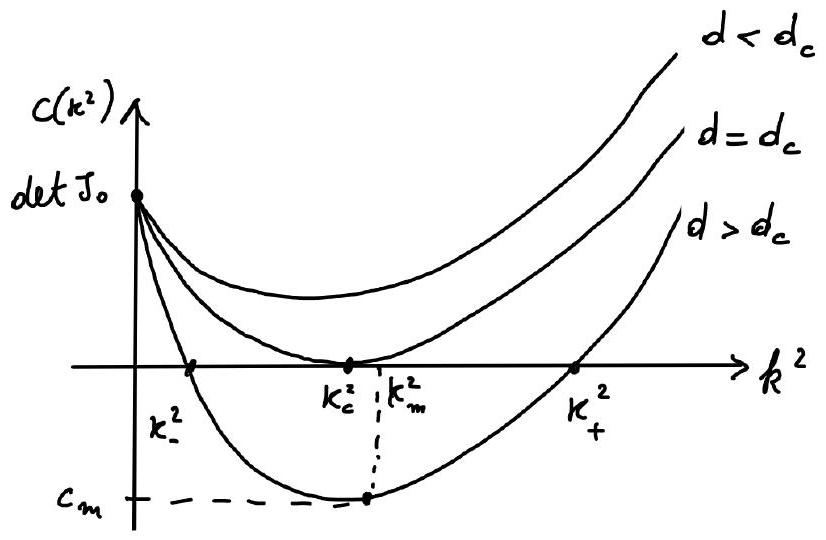
\includegraphics[width=0.5\textwidth]{2025_10_17_3cf351a4349ae3691080g-09}
    \caption{critical diffusivities ratio for Turing patterns to emerge.}
\end{figure}

\subsection*{Critical ratio ($d_c$)}
At the bifurcation $C_{\text {min }}=0$, which can be obtained only when $D_{1}$ and $D_{2}$ have a specific ratio. From eq. (20) and $\frac{D_{2}}{D_{1}}=d$ we get
\begin{DispWithArrows}
    \left(d \partial_{u} f+\partial_{v} g\right)^{2} \geqslant 4 d \operatorname{det} J_{0}>0
\end{DispWithArrows}
So the critical ratio $d_{c}$ of diffusivities satisfies the equation
\begin{DispWithArrows}
    d_{c}^{2}\left(\partial_{u} f\right)^{2}+\left(\partial_{v} g\right)^{2}+2 d \partial_{u} f \partial_{v} g-4 d\left(\partial_{u} f \partial_{v} g-\partial_{v} f \partial_{u} g\right)=0
\end{DispWithArrows}
or
\begin{DispWithArrows}[tag=21]
    d_{c}^{2}\left(\partial_{u} f\right)^{2}+2\left(2 \partial_{v} f \partial_{u} g-\partial_{u} f \partial_{v} g\right) d_{c}+\left(\partial_{v} g\right)^{2}=0
\end{DispWithArrows}
From $d_{c}$ we can calculate the critical wavenumber $k_{c}^{2}$. Indeed from eq. (19)
\begin{DispWithArrows}
    k_{\text {min }}^{2}=\frac{D_{2} \partial_{u} f+D_{1} \partial_{v} g}{2 D_{1} D_{2}}=\frac{1}{D_{1}} \frac{d \partial_{u} f+\partial_{v} g}{2 d}=\frac{1}{D_{1}} \sqrt{\frac{\operatorname{det}\left(J_{0}\right)}{d}}
\end{DispWithArrows}
from eq. (18) with $c_{\text {min }}=0$
from which we obtain (when $c_{\text {min }}=0, k_{\text {min }}=k_{c}$ ):
\begin{DispWithArrows}[tag=22]
    k_{c}^{2}=\frac{1}{D_{1}} \sqrt{\frac{\operatorname{det}\left(J_{0}\right)}{d_{c}}}
\end{DispWithArrows}
where $d_{c}$ is from (21).

\subsection*{Conditions for Turing patterns to emerge}
Conditions (14), (15) and (20) ensure that the spatially uniform state is linearly stable but has at least one wave number $k$ for which $\lambda\left(k^{2}\right)$ has positive real part.
When we impose zero-flux boundary conditions, wavenumbers are restricted to $k=\frac{n \pi}{L}$. Therefore there must exist at least one integer value $n=1,2 \ldots$ for which $c\left(k^{2}\right)<0$ (in this case $d>d_{c}$). In this case the range of unstable wavenumbers is obtained from the zeros $k_{\pm}^{2}$ of $c\left(k^{2}\right)=0$ (see eq. (17)). We get
\begin{DispWithArrows}[tag=22]
    k_{\pm}^{2}=\frac{D_{2} \partial_{u} f+D_{1} \partial_{v} g \pm \sqrt{\left(D_{2} \partial_{u} f+D_{1} \partial_{v} g\right)^{2}-4 D_{1} D_{2}\left(\partial_{u} f \partial_{v} g-\partial_{v} f \partial_{u} g\right)}}{2 D_{1} D_{2}}
\end{DispWithArrows}
\begin{DispWithArrows}[tag=23]
    k_{-}^{2} \leqslant\left(\frac{n \pi}{L}\right)^{2} \leqslant k_{+}^{2}
\end{DispWithArrows}
see also the previous figure and this one
\begin{figure}[H]
    \centering
    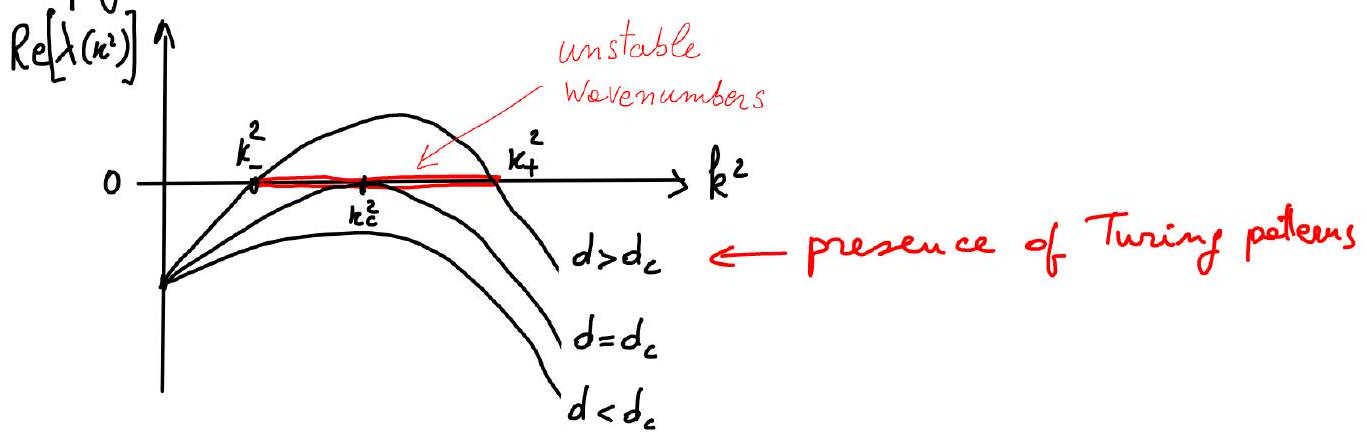
\includegraphics[width=0.5\textwidth]{2025_10_17_3cf351a4349ae3691080g-10}
\end{figure}

\subsection*{Important comments:}
\begin{enumerate}
    \item Because $\partial_{u} f+\partial_{v} g<0$ (eq. (14)) and $D_{2} \partial_{u} f+D_{1} \partial_{v} g>0$ (eq. (20)), it follows that $\partial_{u} f$ and $\partial_{v} g$ must be of opposite sign.
    If we take $\partial_{u} f>0$ (activator) and $\partial_{v} g<0$ (inhibitor) we get $\partial_{u} f<\left|\partial_{v} g\right|$. From eq. (20) we have $D_{2} \partial_{u} f+D_{1} \partial_{v} g>0$, thus
    \begin{DispWithArrows}[tag=24]
        \frac{D_{2}}{D_{1}}>-\frac{\partial_{v} g}{\partial_{u} f}=\frac{\left|\partial_{v} g\right|}{\partial_{u} f}>1 \Rightarrow D_{2}>D_{1}
    \end{DispWithArrows}
    This is usually summarized by saying that
    The inhibitor must diffuse faster than the activator.
    \item From eq. (14) ($\operatorname{Tr}\left(J_{0}\right)<0$), (15) ($\operatorname{det} J_{0}>0$) and eq. (20), it follows that $J_{0}$ must take one of the two forms: ($u$ activ., $v$ inhib.)
    \begin{figure}[H]
        \centering
        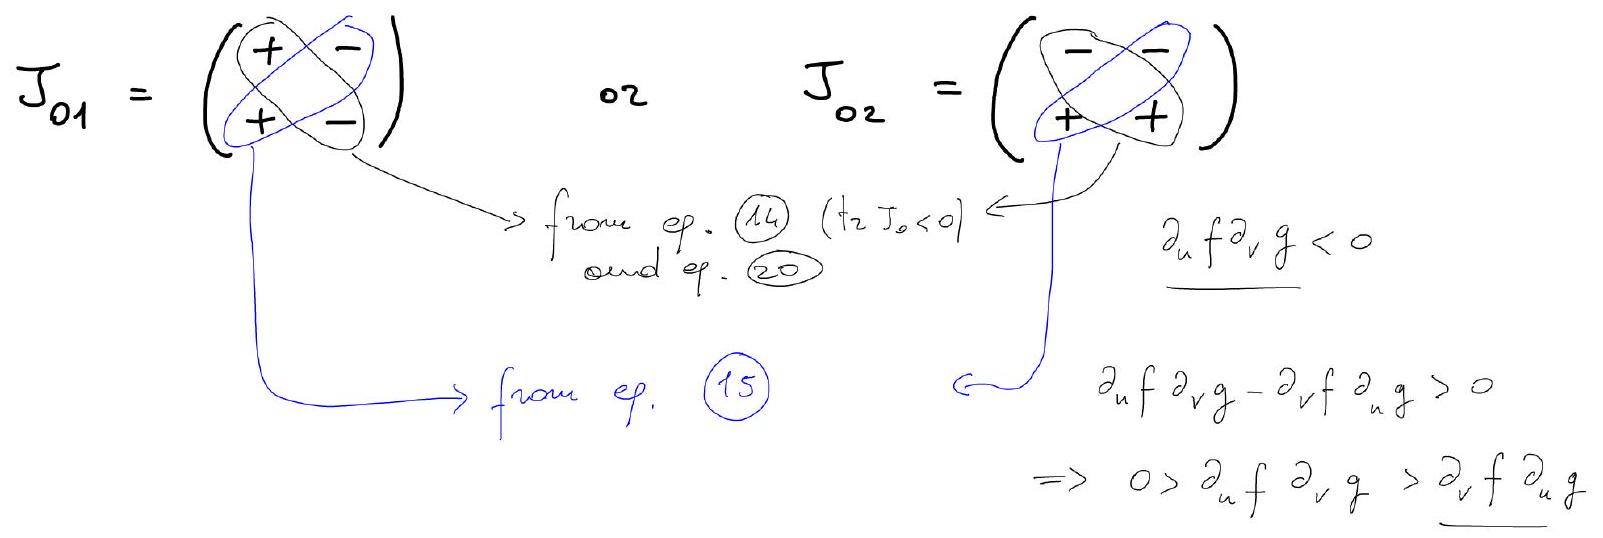
\includegraphics[width=0.5\textwidth]{2025_10_17_3cf351a4349ae3691080g-11}
    \end{figure}
    on the alternative ones ($v$ activ., $u$ inhib.)
    \begin{DispWithArrows}
        J_{03}=-J_{01}=\binom{-+}{-+} \quad J_{04}=-J_{02}=\binom{++}{--}
    \end{DispWithArrows}
    for allowing the emergence of a Turing pattern.
    \item When the linearized equations (see eq. (8)) at $\left(u_{0}, v_{0}\right)$ have $J_{0}$ of the form $J_{01}$, we say that the system is a pure activator-inhibitor system. From eq. (8) and $J_{01}$
    \begin{figure}[H]
        \centering
        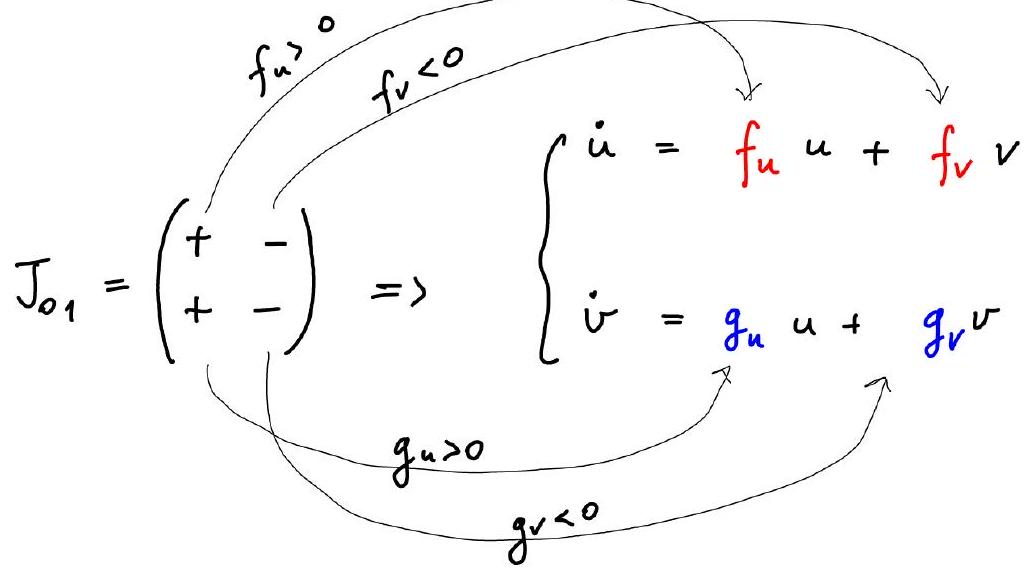
\includegraphics[width=0.5\textwidth]{2025_10_17_3cf351a4349ae3691080g-12(4)}
    \end{figure}
    \begin{figure}[H]
        \centering
        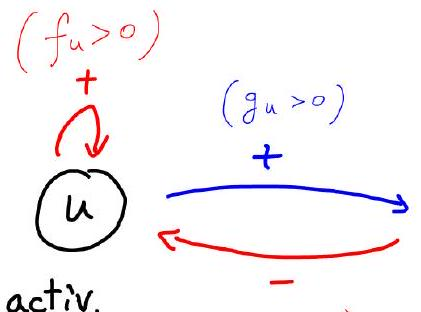
\includegraphics[width=0.5\textwidth]{2025_10_17_3cf351a4349ae3691080g-12}
    \end{figure}
    (a) At steady state $u$ activates its own production, but $v$ inhibits the production of $u$;
    (b) At steady state $u$ also activates the production of $v$, but $v$ inhibits its own production.

    The equations and diagram show why $u$ is termed ACTIVATOR, while $v$ is termed INHIBITOR. Because we also have $D_{2}>D_{1}$ we get short-range activation and long-range inhibition.

    In this case $u$ and $v$ grow in phase: (look at the eigenvectors of $J_{01}$)
    \begin{figure}[H]
        \centering
        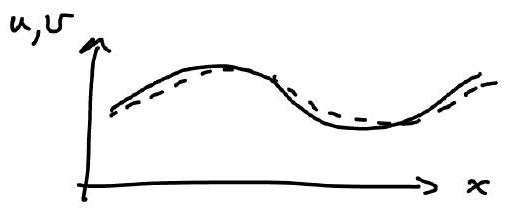
\includegraphics[width=0.5\textwidth]{2025_10_17_3cf351a4349ae3691080g-12(1)}
    \end{figure}
    In the second case for $J_{02}$:
    \begin{figure}[H]
        \centering
        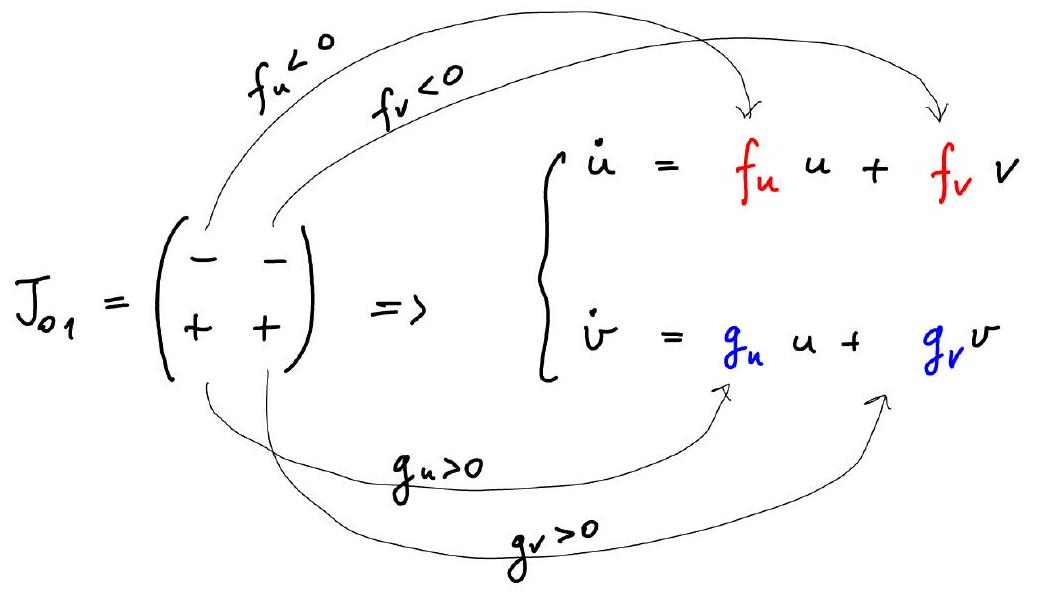
\includegraphics[width=0.5\textwidth]{2025_10_17_3cf351a4349ae3691080g-12(3)}
    \end{figure}
    \begin{figure}[H]
        \centering
        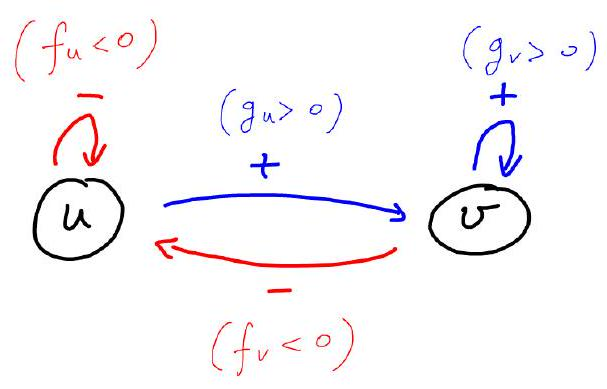
\includegraphics[width=0.5\textwidth]{2025_10_17_3cf351a4349ae3691080g-12(2)}
    \end{figure}
    (c) At steady state, $u$ inhibits its own production as well as $v$ inhibits the production of $u$;
    (d) At steady state, $u$ produces $v$, and $v$ activates itself.

    In this case the system is called cross-activator-inhibitor system and $u$ and $v$ grow out of phase ($180^{\circ}$)
    \begin{figure}[H]
        \centering
        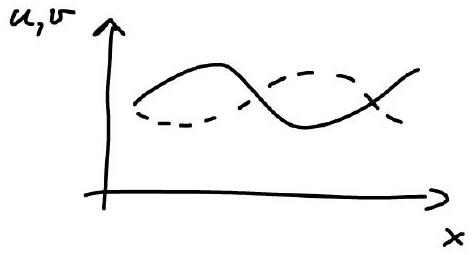
\includegraphics[width=0.5\textwidth]{2025_10_17_3cf351a4349ae3691080g-13}
    \end{figure}
    \item From eq. (23) it follows that there exists a minimum domain size for pattern formation. Indeed, for $L$ sufficiently small, the inequality in (23) cannot be satisfied for $n>0$.
    \item As the domain size increases ($L$ becomes larger), the number of viable integers also increases and the pattern will become more complicated.
    \item Considerations in (3) and (4) can be extended to higher dimensions, where there may occur degeneracy. In $d=2$
    \begin{DispWithArrows}
        k^{2}=\left(\frac{n \pi}{L_{x}}\right)^{2}+\left(\frac{m \pi}{L_{y}}\right)^{2} \quad n, m \in \mathbb{N}
    \end{DispWithArrows}
    Because there may exist multiple pairs ($n, m$) which produce the same $k^{2}$, in higher dimensions different patterns (say, stripes, checkerboard, spots..) may emerge due to different initial conditions, which may combine different solutions (on the basis of the non-linear terms).
\end{enumerate}
